\section{Case study: exact certificate degree beyond flattenings}\label{sec:case}

\subsection{The objective and the resulting theorem}

The case study draws on a complexity research atlas developed during investigations motivated by $\VP_{\C}$ versus $\VNP_{\C}$ \cite{valiant}. Its selected question concerns the degree needed to certify that a tensor has no decomposition with a prescribed number of rank-one terms. The author fixed a standalone objective before the experiments: establish matching upper and lower certificate-degree bounds on an infinite family beyond ordinary flattening tests, using a reusable method.

Before exploration began, the author approved the five acceptance criteria in \cref{tab:case-milestone}. Together they define the case study's completion milestone. Intermediate targets could evolve, while these criteria remained fixed.

\begin{table}[htbp]
\centering\small
\begin{tabularx}{\linewidth}{@{}p{3.8cm}Y@{}}
\toprule
Criterion & Required deliverable \\
\midrule
1. Infinite family & A theorem beyond ordinary flattening tests, with explicit hypotheses and quantifiers in the original decomposition parameters. \\
2. Matching bounds & Matching lower and upper certificate-degree bounds, preferably exact. Matching asymptotics must provide a substantive advance in method and theorem. \\
3. Reusable method & A construction or lower-bound method with a proved extension or justified applicability class beyond one isolated tensor. \\
4. Literature comparison & A documented comparison with the closest tensor-rank and algebraic-proof-complexity results, distinguishing inherited ingredients from the new claims. \\
5. Replayable record & Full arguments, exact checks, source hashes, chronological decisions and failures, and before-and-after reasoning graphs. \\
\bottomrule
\end{tabularx}
\caption{The five prospectively approved criteria for the case study's completion milestone. Completion requires all five.}
\label{tab:case-milestone}
\end{table}

The charter permits a new family to be selected prospectively during exploration. The first family was a sequence of nilpotent matrix pencils; a later target generated from its smallest certificate led to the theorem below.

Let $T\in V_1\otimes\cdots\otimes V_n$, where the $V_i$ are nonzero finite-dimensional complex vector spaces. For a proposed decomposition with $R$ summands, introduce independent parameters $x_{r,i,j}$ and the coefficient equations
\begin{equation}\label{eq:raw-cp}
 F_J(x)=Q_J(x)-T_J,\qquad
 Q_J(x)=\sum_{r=1}^{R}\prod_{i=1}^{n}x_{r,i,j_i},
 \qquad J=(j_1,\ldots,j_n).
\end{equation}
These are the original CP-$R$ equations: CP denotes the decomposition as a sum of completely decomposable, or rank-one, tensors. Their common zero set consists of all such decompositions of $T$. If $\rank(T)>R$, this set is empty. A Nullstellensatz certificate is a polynomial identity
\begin{equation}\label{eq:unit-certificate}
 1=\sum_J h_J(x)F_J(x).
\end{equation}
Define $\delta_R(T)$ as the minimum of $\max_J\deg(h_JF_J)$ over all such identities, with total degree measured in the original parameters. Set $\delta_R(T)=\infty$ when the system has a solution. This convention charges all multiplier costs and specifies the representation in which the theorem holds.

\begin{theorem}[Exact degree for two-term decomposition]\label{thm:main}
Let $n\ge2$ and let $T\in V_1\otimes\cdots\otimes V_n$ have complex tensor rank greater than two. Then
\begin{equation}\label{eq:main-degree}
                       \delta_2(T)=3n.
\end{equation}
The conclusion holds for arbitrary finite mode dimensions, including dimension-one factors.
\end{theorem}

The theorem identifies the first degree at which the full polynomial certificate test can refute every inconsistent two-term decomposition. Its upper bound combines two mechanisms: a flattening minor when one is available, and a transferred boundary certificate otherwise. Its lower bound applies uniformly to the original equations. \Cref{app:math} gives the full argument and the explicit finite identity from which the boundary construction starts.

\subsection{Why the boundary case matters}\label{sec:boundary}

A flattening groups the tensor's modes into two nonempty parts and treats its coefficients as a matrix. A sum of $R$ rank-one tensors has every flattening rank at most $R$. Consequently, a nonzero $(R+1)\times(R+1)$ minor detects excessive rank. The atlas already contained a certificate of degree $n(R+1)$ obtained by telescoping such a minor, together with a lower functional proving that no smaller degree can work for any inconsistent CP-$R$ fiber.

The missing case is a tensor whose exact rank exceeds $R$ while its border rank is at most $R$. Border rank measures membership in the closure of the rank-$R$ tensors. All output polynomials vanishing on rank-$R$ tensors also vanish on that closure. They therefore cannot distinguish such a boundary tensor, whereas its decomposition equations still have no solution. The research target moves from an equation in tensor entries to a unit identity in decomposition parameters. The graph keeps these two objects and their different quantifiers explicit.

For the two-term model, an infinite example is
\begin{equation}\label{eq:wn}
 W_n=\sum_{i=1}^{n}e_0^{\otimes(i-1)}\otimes e_1
                  \otimes e_0^{\otimes(n-i)},\qquad n\ge3.
\end{equation}
Every bipartition $A\mid B$ gives
\[
 W_n=W_A\otimes e_0^{\otimes |B|}
       +e_0^{\otimes |A|}\otimes W_B,
\]
so every flattening has rank at most two. The degeneration
\[
 \frac{(e_0+t e_1)^{\otimes n}-e_0^{\otimes n}}{t}
       \longrightarrow W_n
\]
shows border rank two. Contracting to three active modes yields $W_3$, which has rank three. Thus $W_n$ has no two-term decomposition, and \cref{thm:main} gives the exact degree $3n$ even though all flattening tests at rank two vanish.

\subsection{Starting from the atlas}

At the start of the case study on October 31, the atlas contained 63,494 nodes and 22,183 AND inferences, combining the October 25 extraction with subsequent exploration components. The new run, RRE005, selected the distinct-label functional and flattening certificate from revision 241 of the preceding exploration component, RRE003, retained their source hashes, and rechecked their hypotheses. It began with eight records and no new inference. The initial graph specifies the objective, degree convention, two inherited tools, matrix-pencil baseline, and open boundary question. \Cref{app:complexity-graphs} describes the collection and distinguishes source extraction from subsequent theorem development.

The first chosen tensors have slices
\[
                  T_m=(I_m,J_m),\qquad m\ge2,
\]
where $J_m$ is the nilpotent Jordan block with superdiagonal entries one. Classical matrix-pencil theory gives exact rank $m+1$ and border rank $m$ \cite{buczynskilandsberg}. Here the atlas supplies the lower bound $3(m+1)$, but its flattening upper certificate cannot apply. A short invertible-slice argument verifies the obstruction: an $m$-term decomposition would make $J_m$ similar to a diagonal matrix. This fact establishes the test family; the new quantitative problem is the degree of its unit certificate.

\subsection{From small certificates to a uniform pencil argument}

The first generated task was to make the complete degree test computationally accessible. Each rank-one summand is unchanged by rescaling its mode vectors with scalars whose product is one. Averaging multipliers over these scalings retains only monomials whose degrees are equal across modes within each summand label. Summand permutations provide a further symmetry. This reduction preserves the existence of a certificate at the tested degree, so an unsuccessful complete test has its stated mathematical meaning. It does not discard terms merely because they appear unpromising.

Exact rational elimination found certificates of degrees 9 and 12 for $m=2,3$. Raw-variable expansion checked their identities independently of the orbit multiplication routine. These outcomes generated the sharp-bound target $\delta_m(I_m,J_m)=3m+3$ and a task to exploit the target's additional grading. A modular degree-15 success for $m=4$ was then lifted to a rational certificate and expanded exactly. The three finite values reach the inherited lower bound.

The next generated target sought a uniform proof. For a nonzero nilpotent matrix $N$, choose $H$ with $NH-HN=N$. The decomposition equations and polynomial adjugates produce a commutator identity without dividing by a parameter. Tracking every multiplication yields the following separate result.

\begin{theorem}[Nilpotent-pencil certificate bounds]\label{thm:pencil}
For every $m\ge2$ and every nonzero nilpotent $N\in\C^{m\times m}$,
\begin{equation}\label{eq:pencil-bound}
                3m+3\le\delta_m(I_m,N)\le3m+6.
\end{equation}
The degree is a multiple of three, so it is one of the two displayed endpoints.
\end{theorem}

\Cref{app:pencil} supplies the constructive proof and its degree ledger. This result narrowed an unbounded degree search to one remaining balanced degree block. The graph then generated the exact-endpoint question and retained multiple-block tests with their rational or modular evidence types. For Jordan type $(2,1)$, exact rational elimination places $1$ in the degree-12 row span; type $(2,2)$ passes the degree-15 test over $\mathbb F_{1000003}$. The all-$m$ exact endpoint remains open; that branch retains its own statement when the later two-term theorem is added.

\subsection{Charging contracted modes in a transfer}

The search used a balanced basis from the start: \cref{lem:balance} guarantees that every certificate can be made label-balanced without increasing its degree. The degree-9 identity supplies a concrete base certificate. The useful transfer question is quantitative: if a higher-order tensor contracts to its target, how much degree is needed to pull the identity back in the original parameters? Target T011 records this proposal before the transfer checks and the all-target theorem were saved. The key step is to charge all contracted modes through the existing balance, so a degree block of size $k$ becomes one of size $n$.

The answer is a general lemma. Suppose a $k$-mode CP-$R$ certificate has label-balanced multipliers of degree at most $k(q-1)$. If an $n$-mode target maps to its target by linear maps on $k$ retained modes and linear functionals on the other modes, then the certificate pulls back with product degree at most $nq$ in the original parameters. Contracted parameter factors are absorbed into the first retained mode of each summand. Balance makes a multiplier of degree $kt$ become one of degree at most $nt$; the substituted equation is a constant linear combination of original equations. This is the precise cost that the graph's degree convention requires.

Combining balance reduction with the transfer lemma removes any separate balance assumption on the certificate. If $T$ has order $n$, $S$ has order $k\le n$, and $T$ maps to $S$ by the stated mode maps and contractions, then
\[
 \delta_R(T)\le\frac{n}{k}\,\delta_R(S),\qquad \delta_R(S)<\infty.
\]
\Cref{cor:degree-transfer} proves this general bound by applying transfer to a minimum-degree certificate. It makes the method reusable for every finite CP-$R$ certificate under the specified maps.

The smallest pencil $(I_2,J_2)$ becomes $W_3$ after a coordinate swap. Its degree-9 certificate therefore transfers to $W_n$ with degree $3n$. The inherited lower bound is also $3n$, establishing an exact infinite-family result. The same lemma can now be reused wherever a target has the required contraction. It is the new bridge between a finite polynomial identity and an all-order theorem.

\subsection{From the family to the full two-term model}

The next step combines the transfer with classical geometry. Landsberg and Manivel show that the $3\times3$ minors of all bipartition flattenings define the second Segre secant variety set-theoretically; Raicu proves the stronger ideal-generation result \cite{landsbergmanivel,raicu}. Within this secant variety, a tensor that is not an actual two-term sum lies on a tangent space to the Segre variety \cite[arXiv version, Corollary~1 and Notation~1]{ballicobernardi}. Such a tensor can be written
\begin{equation}\label{eq:tangent-main}
 T=\lambda\bigotimes_i v_i+
       \sum_i u_i\otimes\bigotimes_{j\ne i}v_j,
\end{equation}
with the factors placed in their corresponding modes. Rank greater than two requires at least three active modes, in which $u_i$ is independent of $v_i$. Retaining three of them, contracting the others, and removing the pure term by a constant shear gives $W_3$.

This yields an exhaustive case split. If some flattening has rank greater than two, the minor certificate has degree $3n$. Otherwise, the tangent projection and balanced transfer have degree $3n$. Combining either upper route with the inherited lower bound proves \cref{thm:main}. In the reasoning graph, the two routes are conditional derivations followed by an exhaustive-case inference. They are not two hypotheses that the target must satisfy simultaneously.

The $W_n$ corollary has a shorter prerequisite path: the explicit base identity, the transfer lemma, and the lower functional suffice. The full theorem additionally uses the classical geometric classification. Separate traces expose exactly where those imports enter. The contribution is the original-parameter certificate-degree characterization and its transfer method; the tensor-rank and secant classifications retain their established attribution.

\subsection{Verification and the quantitative record}\label{sec:case-checks}

The proof is accompanied by exact checks at three levels. First, the certificates for the single-block pencils $(I_m,J_m)$, $m=2,3,4$, expand to the constant polynomial one over $\Q$. The largest has 6,211 orbit terms and 429,076 expanded product terms. Second, the commutator identities were checked symbolically for $m=2$ and at 112 exact substitutions across 14 Jordan-block families through $m=8$, including singular parameter matrices. Third, the transferred certificate was expanded in the original $W_n$ variables for 32 orders, $n=3,\ldots,32,64,128$. All identities equal one and have degree $3n$. A further 288 exact coefficient-map identities test contraction, nontrivial basis changes, and removal of the pure tangent term across 36 cases.

These computations test the explicit certificates and their implementations; the uniform conclusions follow from the proofs in \cref{app:math}. A modular success is retained as a modular result until a rational certificate is supplied. Mathematical arguments, exact identities, classical imports, and structural validation have separate records. The study includes internal mathematical review, exact replay, and an initial audit of the mathematical arguments by the author. Its literature comparison concerns the specific certificate-degree statement and the primary works described above.

The closest existing formulations clarify the advance. Tensor-rank Nullstellensatz systems were already available \cite{aliabadifriedland}; the present theorem gives a sharp threshold for their original two-term equations. The flattening equations describe a closure in tensor space \cite{landsbergmanivel,raicu}; the boundary certificate instead proves emptiness of an exact decomposition fiber. The secant--tangent dichotomy supplies the exhaustive cases \cite[arXiv version, Corollary~1]{ballicobernardi}; the balanced lemma supplies the parameter-degree bound. These are distinct contributions in the dependency graph.

\subsection{Graph evolution, replay, and visualization}\label{sec:visual-effects}

Six immutable versions record the investigation. The graph grows from eight records to 68 nodes and 34 AND inferences. Each publication retains a delta and source hashes and advances the new component in the atlas. The final version records acceptance against the original infinite-family objective. A 44-record event history preserves target proposals, computations, proofs, corrections, publication events, and the stopping decision. \Cref{app:records} explains the event identifiers and replay procedure.

\begin{table}[htbp]
\centering\small
\begin{tabularx}{\linewidth}{@{}p{1.4cm}r r Y@{}}
\toprule
Revision & Nodes & AND steps & Mathematical or historical effect \\
\midrule
v001 & 8 & 0 & Fix the objective, raw model, inherited bounds, and boundary family. \\
v002 & 19 & 7 & Establish complete symmetry reduction and exact degrees 9 and 12; generate a uniform target. \\
v003 & 43 & 22 & Certify degree 15 and prove the all-$m$ pencil bound; generate the endpoint question. \\
v004 & 46 & 22 & Add multiple-block screens and retain the remaining gap. \\
v005 & 66 & 33 & Prove balanced transfer, the $W_n$ formula, and the all-target two-term theorem. \\
v006 & 68 & 34 & Complete the mathematical audit, replay delivery, and milestone assessment. \\
\bottomrule
\end{tabularx}
\caption{Saved graph states during the exploration. Counts include scopes, evidence, objectives, and open questions as well as derived claims.}
\label{tab:versions}
\end{table}

\begin{figure}[p]
\centering
\begin{tikzpicture}[>=Latex,font=\small,
 card/.style={draw=blue!40!black,rounded corners=3pt,fill=blue!3,align=left,text width=5.65cm,minimum height=2.3cm,inner sep=9pt},
 arr/.style={->,thick,draw=blue!55!black}]
\node[card] (a) at (0,0) {\textbf{1. A gap in inherited reasoning}\\[3pt]
Lower degree $n(R+1)$; the matching upper certificate needs a large flattening.\\[3pt]\footnotesize v001: 8 nodes, 0 new inferences};
\node[card] (b) at (7.1,0) {\textbf{2. Boundary certificates}\\[3pt]
Symmetry makes complete tests feasible. Exact degrees 9 and 12 suggest a uniform target.\\[3pt]\footnotesize v002: 19 nodes, 7 inferences};
\node[card] (c) at (0,-3.4) {\textbf{3. A uniform pencil theorem}\\[3pt]
Adjugates and a commutator give\\$3m+3\le\delta_m\le3m+6$.\\[3pt]\footnotesize v003: 43 nodes, 22 inferences};
\node[card] (d) at (7.1,-3.4) {\textbf{4. Retain the remaining question}\\[3pt]
Multiple-block tests preserve the exact endpoint as open. The base identity remains reusable.\\[3pt]\footnotesize v004: 46 nodes, 22 inferences};
\node[card,fill=green!5] (e) at (0,-6.8) {\textbf{5. Charge contracted modes}\\[3pt]
Transfer costs the factor $n/k$. The degree-9 base and geometry give $\delta_2(T)=3n$.\\[3pt]\footnotesize v005: 66 nodes, 33 inferences};
\node[card,fill=green!5] (f) at (7.1,-6.8) {\textbf{6. Publish and preserve}\\[3pt]
Audit the original criteria; save proofs, checks, graph paths, and further targets.\\[3pt]\footnotesize v006: 68 nodes, 34 inferences};
\draw[arr] (a)--(b);
\draw[arr] (b.south)--($(b.south)!0.5!(d.north)$)-| (c.north);
\draw[arr] (c)--(d);
\draw[arr] (d.south)--($(d.south)!0.5!(f.north)$)-| (e.north);
\draw[arr] (e)--(f);
\end{tikzpicture}
\caption{Recorded research progression. Each stage changes what the next investigation can use. Arrows describe exploration history, while the theorem's implication structure is shown separately in \cref{fig:certificate-proof}. The open pencil endpoint survives the success of the two-term branch.}
\label{fig:discovery-timeline}
\end{figure}

\begin{figure}[p]
\centering
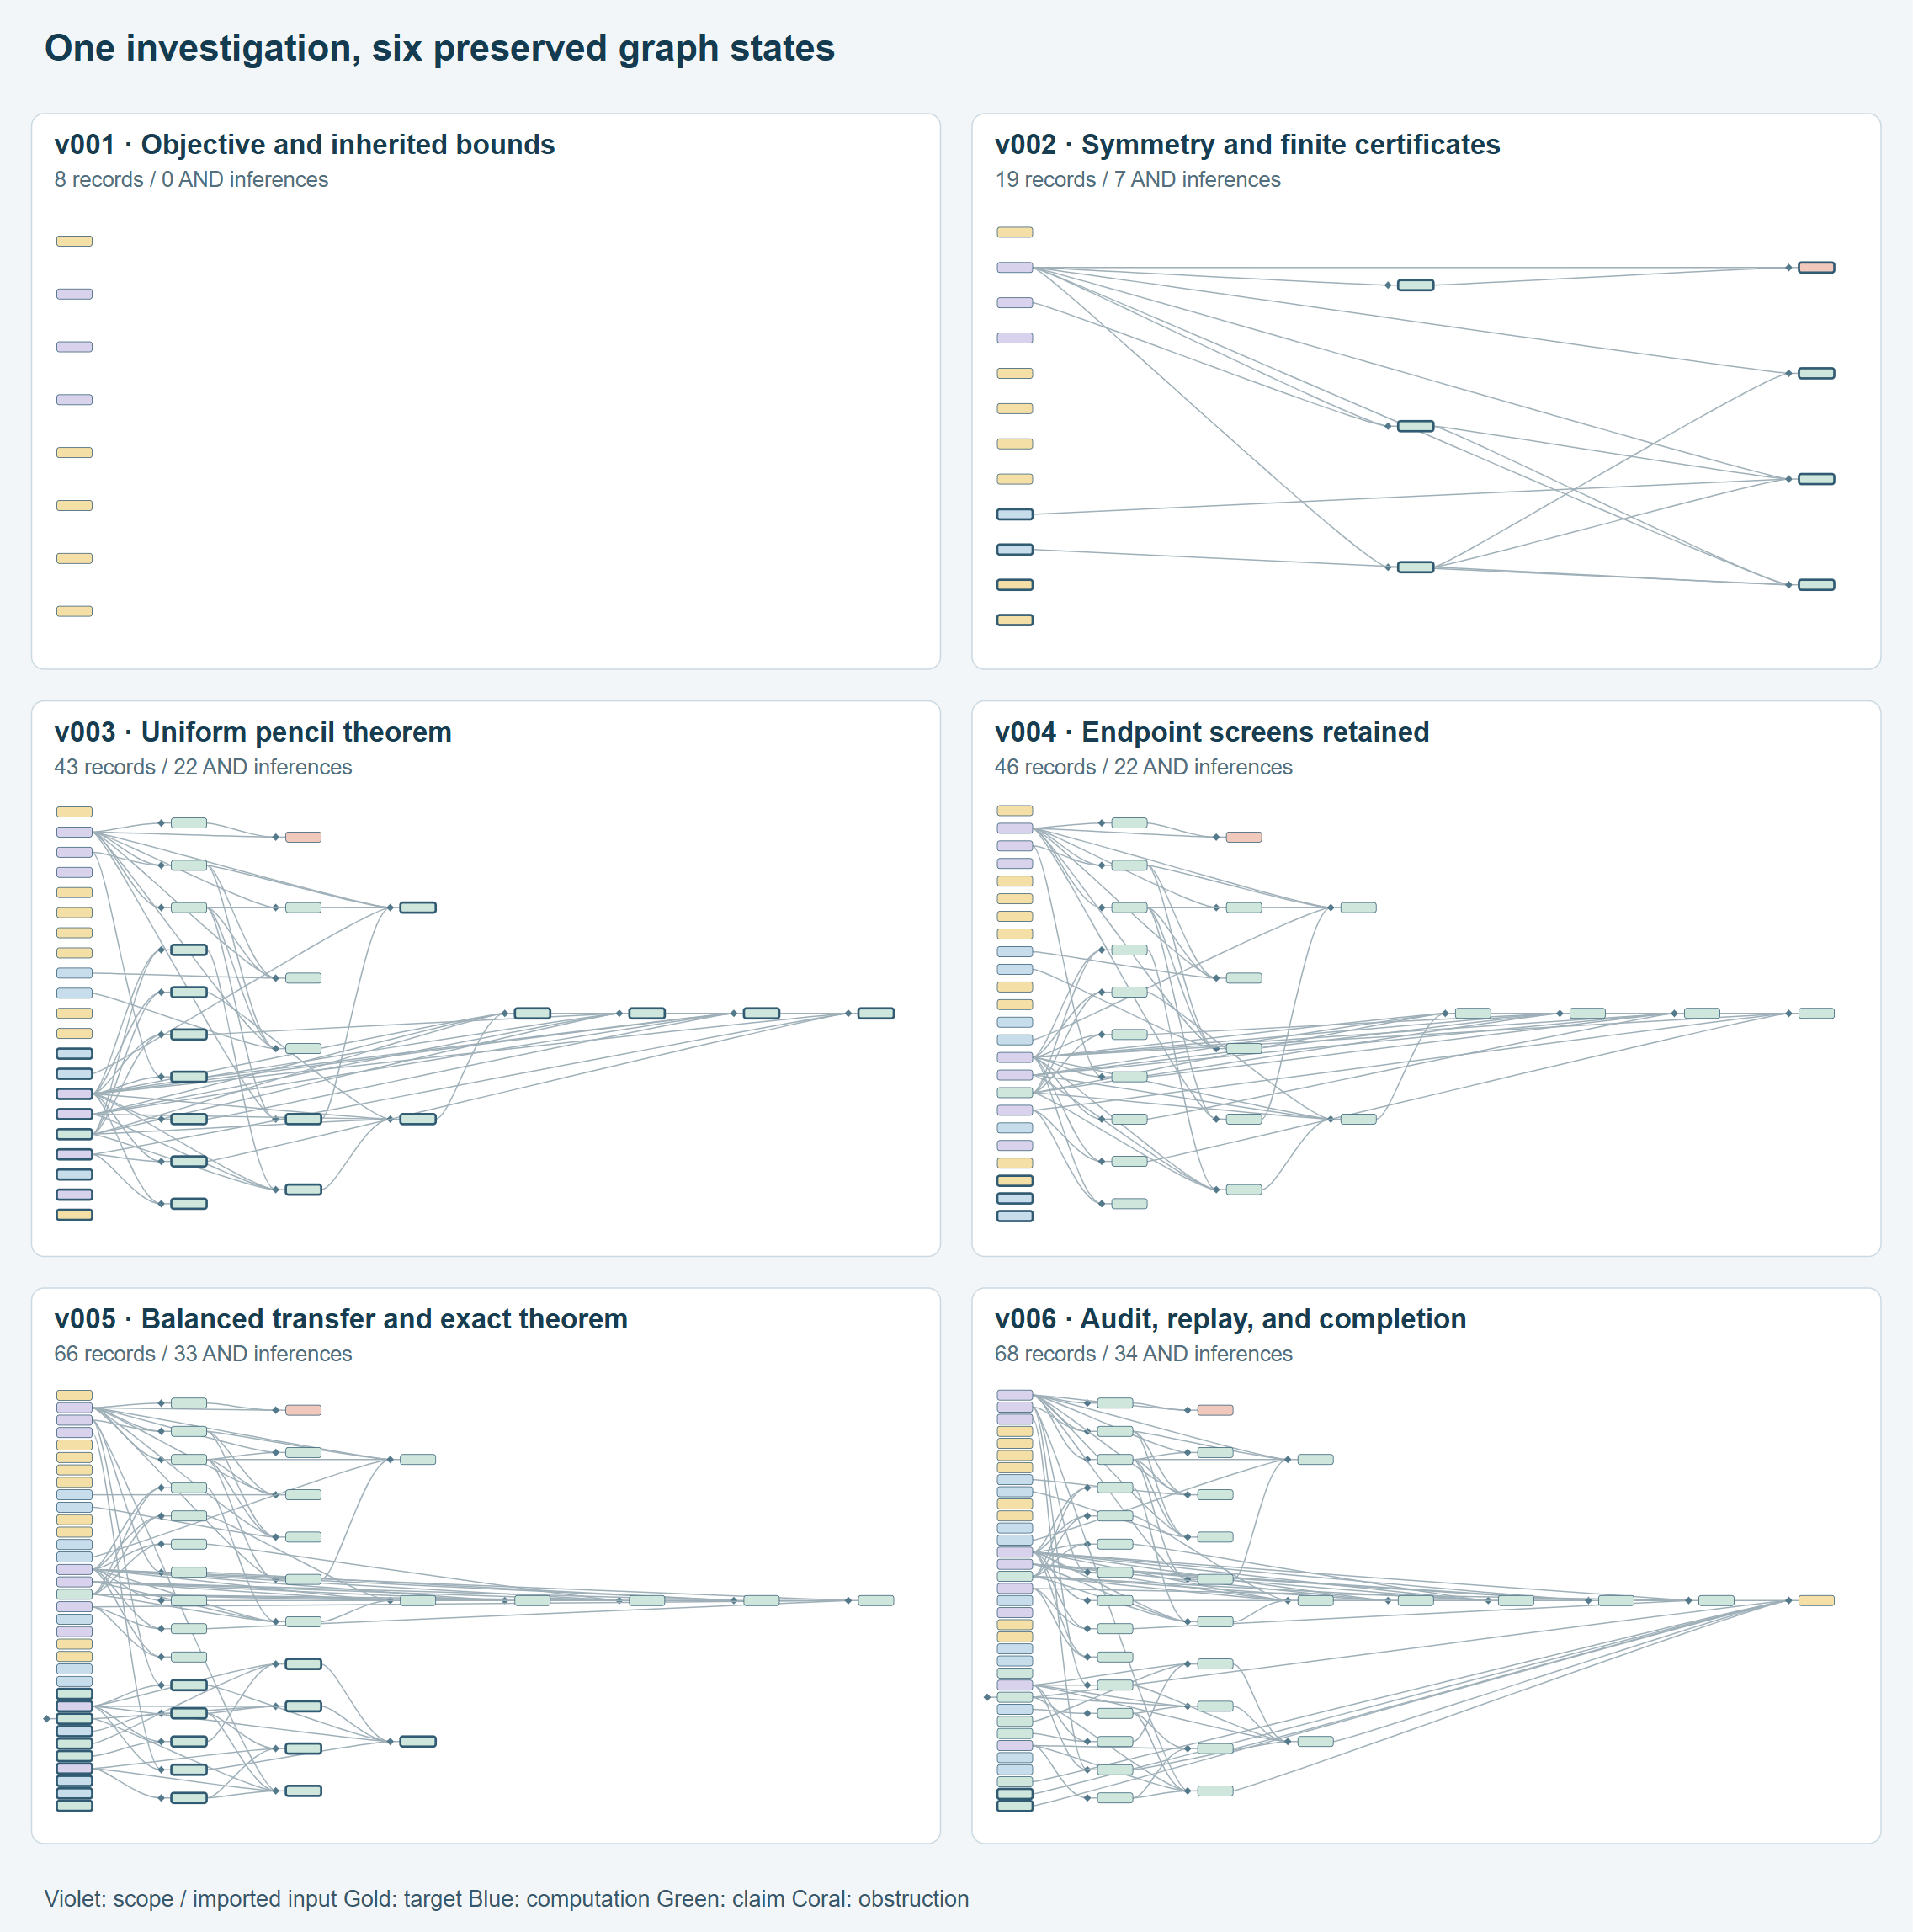
\includegraphics[width=\linewidth]{figures/certificate_degree/versions.png}
\caption{Incremental growth of the certificate-study graph, rendered from the six saved graph files. Each small map contains all records and inference segments in that version; positions follow proof depth, and scopes, targets, computations, and claims retain different colors. After v001, heavier outlines mark newly added records. Counts measure records, not independent theorems. The compact maps show structure; the companion opens each version at full resolution with statements and evidence.}
\label{fig:certificate-versions}
\end{figure}

\begin{figure}[p]
\centering
\begin{tikzpicture}[>=Latex,font=\small,
 box/.style={draw=blue!40!black,rounded corners=2pt,align=center,text width=5.55cm,minimum height=1.45cm,inner sep=8pt,fill=blue!3},
 result/.style={box,fill=green!6,draw=green!40!black},
 arr/.style={->,draw=blue!55!black,thick}]
\node[box,text width=12.5cm,fill=violet!5] (scope) at (3.5,0)
 {\textbf{Scope:} order $n\ge2$, tensor rank $>2$, over $\C$\\Original two-term equations; total multiplier--equation degree};
\node[box] (split) at (3.5,-2.2) {\textbf{Exhaustive cases}\\Some flattening rank $>2$, or every flattening rank $\le2$};
\node[box] (minor) at (0,-4.6) {\textbf{Case A: inherited minor lemma}\\A nonzero $3\times3$ minor\\gives an upper certificate of degree $3n$};
\node[box] (geom) at (7,-4.6) {\textbf{Case B: classical geometry}\\Secant-two flattening theorem\\and tangent-space description};
\node[result] (transfer) at (7,-7.0) {\textbf{Projection and balanced transfer}\\Map the target to $W_3$; pull back\\the explicit degree-9 certificate};
\node[result] (upper) at (3.5,-9.3) {\textbf{Upper bound in every case}\\$\delta_2(T)\le3n$};
\node[box] (lower) at (0,-7.0) {\textbf{Inherited lower functional}\\Annihilates $h_JF_J$ when\\$\deg(h_JF_J)<3n$, but $L(1)=1$};
\node[result,text width=8cm] (exact) at (3.5,-11.7) {\textbf{Exact theorem}\\$\delta_2(T)=3n$ for every $\rank(T)>2$};
\draw[arr] (scope)--(split);
\draw[arr] (split.west)-|(minor.north);
\draw[arr] (split.east)-|(geom.north);
\draw[arr] (geom)--(transfer);
\draw[arr] (minor.west)--++(-.45,0)|-(upper.west);
\draw[arr] (transfer.south)|-(upper.east);
\draw[arr] (upper)--(exact);
\draw[arr] (lower.south)--++(0,-.7)--++(-3.3,0)|-(exact.west);
\end{tikzpicture}
\caption{Proof outline of the exact theorem, with the original-parameter scope attached throughout. Blue boxes denote inherited or classical inputs; green boxes show the certificate transfer and resulting bounds. The two upper routes are conditional arguments combined by exhaustive cases; for $n=2$, only Case A occurs. The lower functional and either applicable upper route yield equality. Each box summarizes the indicated lemma or argument in \cref{app:math}; the companion expands its recorded premises.}
\label{fig:certificate-proof}
\end{figure}

\begin{figure}[p]
\centering
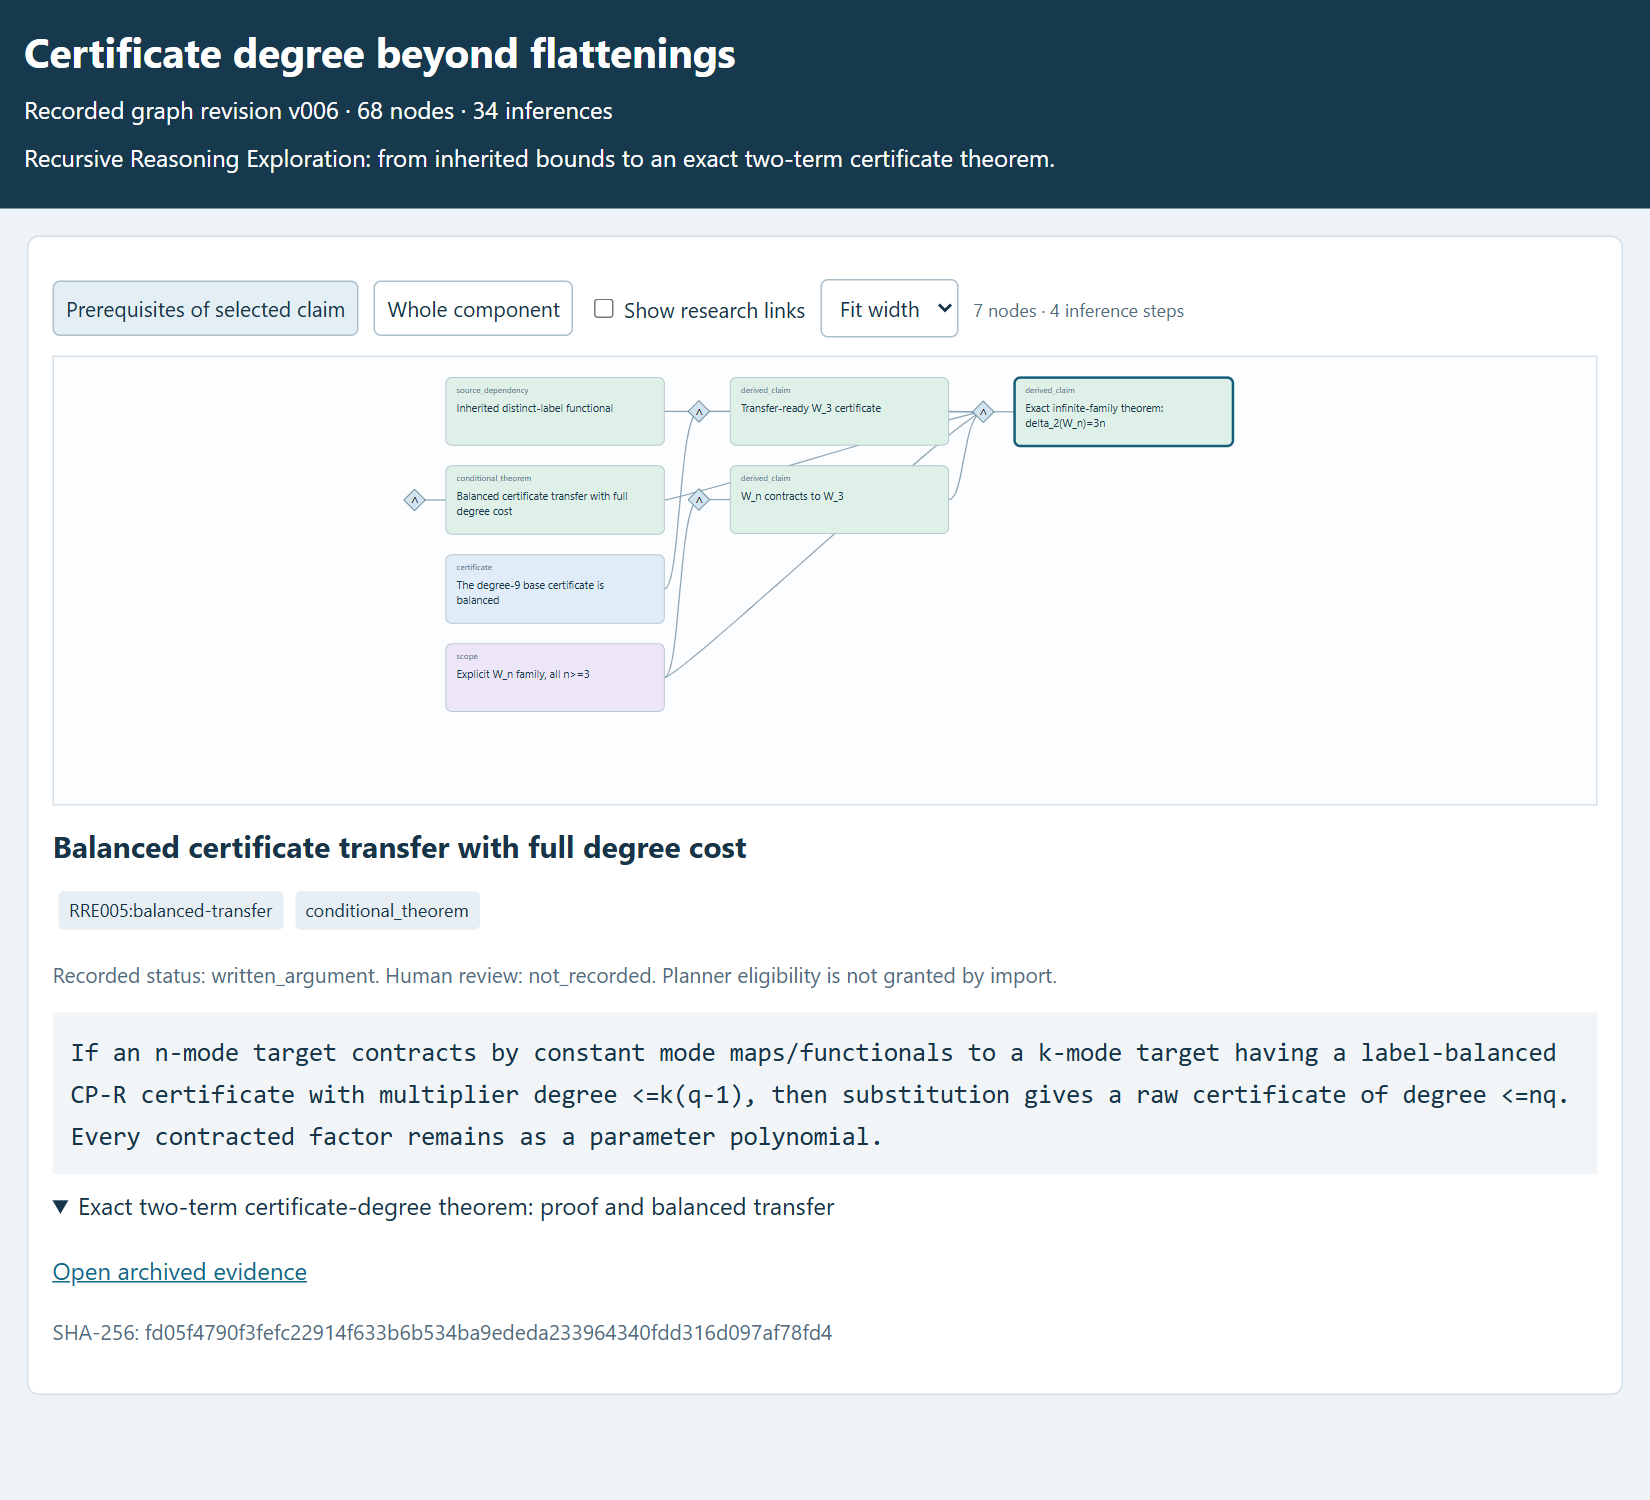
\includegraphics[width=\linewidth,height=.75\textheight,keepaspectratio]{figures/certificate_degree/inspector.png}
\caption{The implemented companion connects a selected graph record to its statement, scope, and hash-pinned evidence. The view focuses on the balanced transfer used to extend the boundary certificate. It is an interface excerpt; the versioned companion provides the full graph and prerequisite traces.}
\label{fig:certificate-inspector}
\end{figure}


The companion provides a view for every saved version and prerequisite traces for each result. The six-version overview in \cref{fig:certificate-versions} shows how the argument grows from the inherited input. \Cref{fig:certificate-proof} summarizes the proof routes and their scope, while \cref{fig:certificate-inspector} shows the evidence inspector. The companion exposes the individual AND steps and attached hypotheses. The timeline in \cref{fig:discovery-timeline} instead shows how mathematical outcomes generated subsequent targets. Distinguishing these views lets a reader reconstruct both the final proof and the recorded process that produced it.

Two dedicated exports retain the nilpotent-pencil and exact two-term theorem paths with their evidence. They can be consumed by a separate visualization process while exploration continues elsewhere in the atlas. The final component is integrated, while the earlier working graphs and their revisions remain intact.

\subsection{What the case contributes to the RRE method}

The case has several recursive transitions with explicit mathematical content. Finite certificates generate a uniform theorem target; its additive gap generates an endpoint question; the question of charging contracted modes generates a transfer target; and the transfer combines with classical geometry to cover every inconsistent two-term fiber. The record retains why each question became useful and which premises made the resulting answer valid.

The decisive change of viewpoint is also preserved. A tensor in a rank closure cannot be excluded by an output equation, yet its empty exact decomposition fiber admits a polynomial certificate. Recording this distinction avoids repeatedly pursuing the wrong type of obstruction. Recording the base identity, the general balance reduction, and the contraction degree calculation makes the later reuse inspectable. The theorem and the reusable bridge supply the substantive mathematical outcome; the evolving graph supplies an inspectable account of their dependencies and development. 

The final results meet the criteria in \cref{tab:case-milestone} as follows. The exact formula $\delta_2(W_n)=3n$ for every $n\ge3$ supplies an infinite family beyond flattenings with matching bounds (criteria 1 and 2); \cref{thm:main} extends this to the full two-term model. The general transfer lemma supplies the reusable method (criterion 3). The comparison in \cref{sec:case-checks} identifies the contribution relative to prior work (criterion 4). The proofs, exact checks, pinned sources, event history, and six graph revisions provide the replayable record (criterion 5). These deliverables support the completion decision recorded in the final revision. The comparative value of this organization is the subject of the evaluations proposed next.
